
\subsection{Tasks Correctness}
\label{cp6:correctness}



When assisted by a tool able to automatically highlight text identified as relevant to a task, we expect that a developer can produce a solution 
that is equally or more correct than the solution of a developer who attempted a task without tool support. 


To compute how correct a participant's solution is, 
we compile their submitted code and run it against a set of 10 test cases that check whether it produces the correct output for each given test input. 
Hence, \textit{correctness} represents the number of passing test cases of a solution (Equation~\ref{eq:cp6-correctness}).
For example, if the solution of a participant passes 7 out of 10 test cases, we would assign a 
correctness score of $7$ to this solution. 
A solution with compile errors has a correctness score of $0$.


\begin{small}
\begin{equation}
    Correctness = \text{\textit{\# of passing test cases}}
    \label{eq:cp6-correctness}
\end{equation}
\end{small}



From all submitted solutions (24 manual and 24 tool-assisted ones), two 
solutions from tool-assisted tasks had compile errors or failed all test cases. 
One of these
was from a participant who indicated that they decided to not finish their tool-assisted task due to time constraints; 
the other, from an exception thrown in the code of a participant who misused the \texttt{geopy} module. We do not ignore these two solutions when reporting results.



\subsubsection{Results}


Figure~\ref{fig:correctness-overall} aggregates all correctness scores for tasks done with and without tool support.
Although we observe that there is less variability in the solutions of participants assisted by our tool,
we cannot draw statistically significant conclusions based on the data for correctness~\cite{Lazar2017-cp3}.
Hence, we evaluate scores on a per task basis, as shown in Figure~\ref{fig:correctness-by-task}.



\medskip
\begin{figure}[h!]
    \centering
    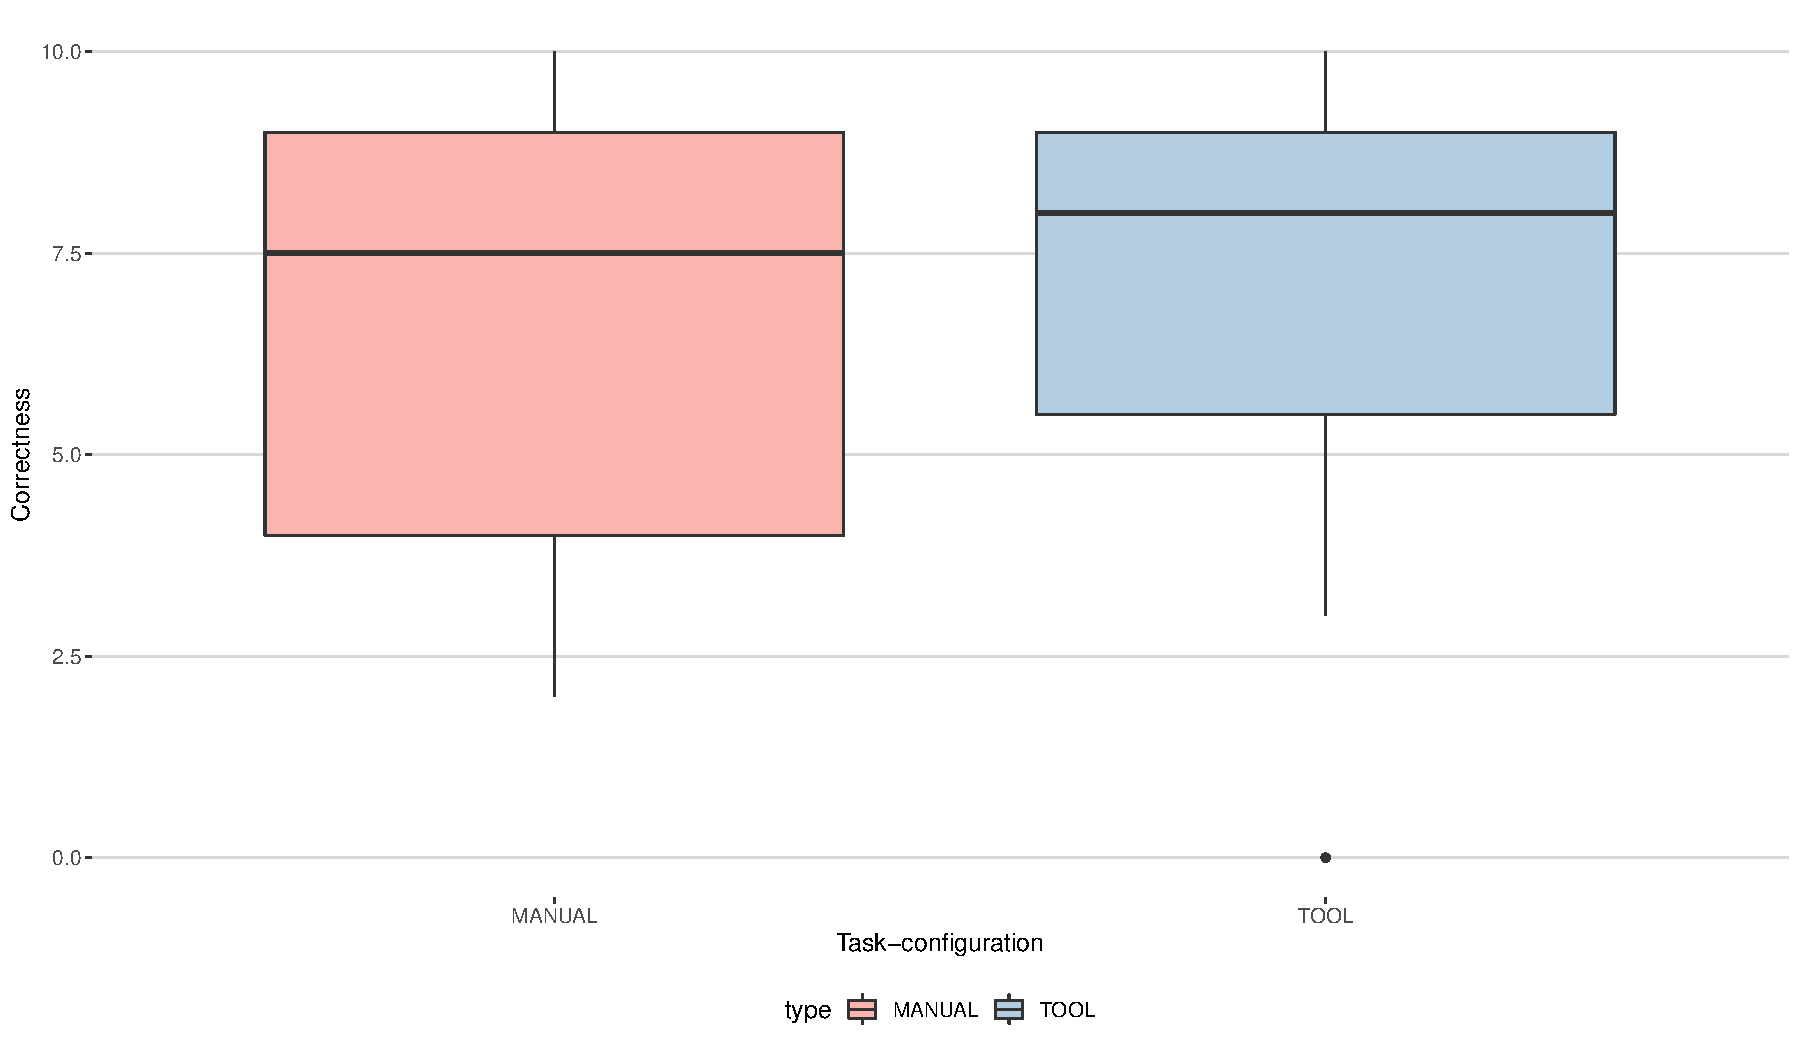
\includegraphics[width=0.8\textwidth]{cp6/correctness_aggregated.pdf}
    \caption{Boxplots showing aggregated correctness scores for task performed with and without tool support}
    \label{fig:correctness-overall}
\end{figure}




Comparing the correctness scores of solutions submitted by participants
who performed each task with and without tool support, we observe that participants with tool support performed worse in the \texttt{distances} task. 
Among potential reasons for the lower score, we believe that the text automatically identified 
might not have been relevant for this task, what can explain the higher percentage of participants
who indicated that the text identified  by the tool was indeed not helpful (Section~\ref{cp6:usefulness}).



Manual and tool-assisted solutions have the exact same correctness distribution in \texttt{NYTimes} tasks.
We found that the most notable differences in the solutions of this task arised from participants who did (or not) consider corner-case scenarios.
To illustrate this, we quote one participant who stated that their solution could ``\textit{fetch all the articles, but it could also get some noise}'',
e.g., getting all the headlines of the web page but also an unrelated ad, which is indeed one of the test cases for this task. 



The \texttt{titanic} task required using two python modules and it is the one with the most differences. 
Participants who did the task with tool support were able to produce more correct solutions, with an average 
correctness score of $6$. In contrast, participants in the control group had an average correctness of $4$. 
As we detail in the next sections, we found that the text automatically identified for this task 
was considered the most useful and that the tool identified much of the text that humans deemed relevant. 





\begin{figure}
    \centering
    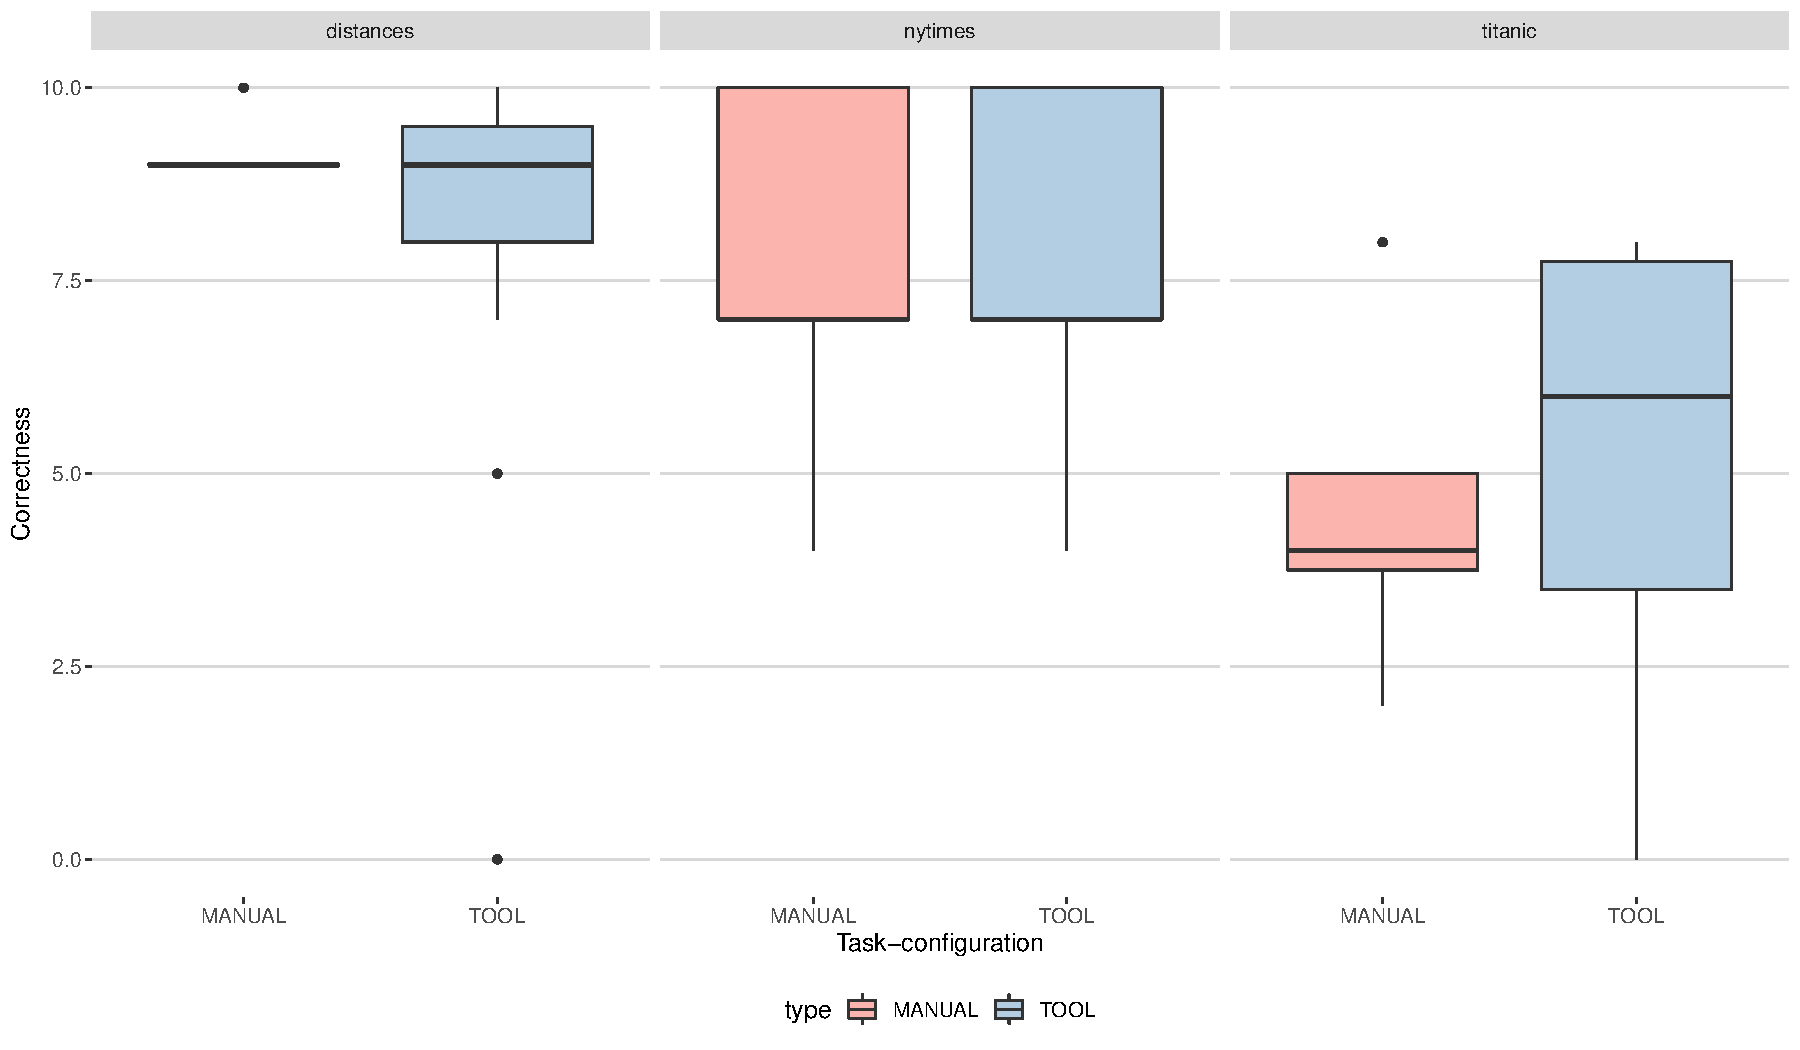
\includegraphics[width=\textwidth]{cp6/correctness_overall.pdf}
    \caption{Boxplots showing correctness scores for each task performed with and without tool support}
    \label{fig:correctness-by-task}
\end{figure}




